% Drawing 45/04-1 -- folder 45, batch 04, archive page 78 (PDF page 79).
% Transcription: en haut à droite, un petit dessin barré portant « $x^2 = a$ », « $x^2 - a + y^2 = 0$ » et « $x/t$ »
% Kind: small struck sketch with equations. Method 2 (schematic redraw from the facsimile). Status: partial.
% Notes: A vertical stroke with the labels "x^2 = a", "x^2 - a + y^2 = 0" and "x/t" beside it, as the transcription reads them, and the scribble striking it (drawn grey, schematised). A label on the left of the stroke is left out (not read).
% Coordinates: 1 unit = 1 mm = 1/100 of the crop width (bbox in page fractions: [0.8, 0.07, 0.96, 0.17]).
% Redrawn by Claude (claude-opus-5-5), issue #73, 2026-11-07; not checked by a human; not compiled (no TeX in the session).
% Rights: reproduces part of the work -- behind RENDER_TRANSCRIPTS, never published by itself.
\documentclass[tikz,border=3pt]{standalone}
\usepackage{amsmath,amssymb}
\usetikzlibrary{patterns,arrows.meta}
\tikzset{pencil/.style={black!45}, struck/.style={black!35}, mark/.style={circle,draw,inner sep=1.3pt}, pt/.style={circle,fill,inner sep=0.9pt}, opt/.style={circle,draw,fill=white,inner sep=1.1pt}}
\begin{document}
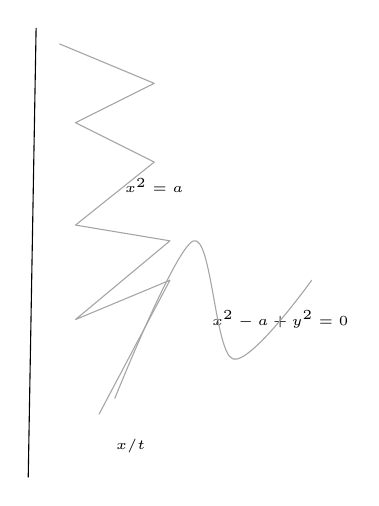
\begin{tikzpicture}[x=1mm,y=1mm,line cap=round,line join=round,font=\scriptsize]
\draw (25,-13) -- (24,-70);
\node[inner sep=1pt] at (40,-33) {\tiny $x^2=a$};
\node[inner sep=1pt] at (56,-50) {\tiny $x^2-a+y^2=0$};
\node[inner sep=1pt] at (37,-66) {\tiny $x/t$};
\draw[struck] (28,-15) -- (40,-20) -- (30,-25) -- (40,-30) -- (30,-38) -- (42,-40) -- (30,-50) -- (42,-45) -- (33,-62);
\draw[struck] plot[smooth, tension=0.55] coordinates {(35,-60) (45,-40) (50,-55) (60,-45)};
\end{tikzpicture}
\end{document}
